\begin{tikzpicture}
\node[anchor=south west,inner sep=0] at (-\muonroutd-.125, -\muonroutd-.125) {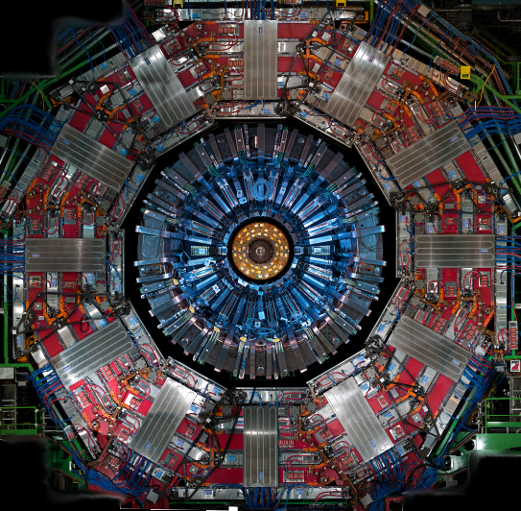
\includegraphics[width=15 cm]{\PhDthesisdir/plots_and_images/CMS_zoomout_pictures/CMS_slice_photo_6-muons.png}};

\begin{scope}
\clipSlice

\drawCMS

\printphotondeposit{35}
\printphotonnolabel{35}
%\printphotonlabel{15}

\printantimuondeposit{7}{15}
\printantimuonnolabel{7}{15}
\printantimuontrk{7}{15}

\printeledeposit{3.5}{-50}
\printelenolabel{3.5}{-50}
\printeletrk{3.5}{-50}

\printneutralhadrondeposit{15}
\printneutralhadronnolabel{15}

\printhadrondeposit{7}{-15}
\printhadronnolabel{7}{-15}
\printhadrontrk{7}{-15}
\end{scope}

\end{tikzpicture}